\documentclass[tikz, border=0.2cm]{standalone}

\begin{document}
	
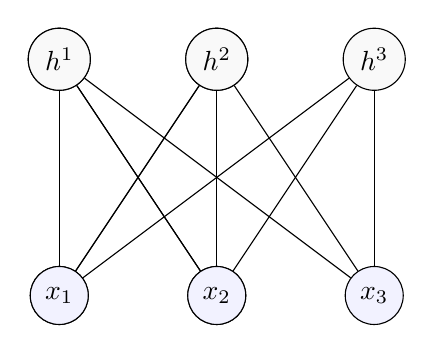
\begin{tikzpicture}
\tikzset{
	node/.style = {
		draw, circle, 
		fill=blue!5
	},
	hmid/.style={
		fill=gray!5
	},
	every edge/.style={
		draw, thin
	},
}

% manual labor
\node [node, hmid] (h1) at (2, 3) {  $h^1$ };
\node [node, hmid] (h2) at (4, 3) {  $h^2$ };

\node [node] (x1) at (2, 0) {$x_1$};
\node [node] (x2) at (4, 0) {$x_2$};

\path (h1) edge [draw] (x1);
\path (h1) edge [draw] (x2);
\path (h2) edge [draw] (x1);
\path (h2) edge [draw] (x2);


% draw the nodes 
\foreach \i in {1,...,3}
{
  \node[node, hmid] (h\i) at (\i*2, 3) {$h^\i$};
  \node[node] (x\i) at (\i*2, 0) {$x_\i$};
}


% attach them 
\foreach \i in {1,...,3}{
  \foreach \v in {1,...,3}{
    \path (h\i) edge (x\v);
  }
}


\end{tikzpicture}
	
	
\end{document}
